\documentclass[11 pt]{scrartcl}
\usepackage[header, margin, koma, stylish]{tyler}

\newcommand{\hwtitle}{Discussion 3B Recap}

\pagestyle{fancy}
\fancyhf{}
\fancyhead[l]{\hwtitle{}}
\fancyhead[r]{Tyler Zhu}
\cfoot{\thepage}

\begin{document} 
\title{\Large \hwtitle{}}
\author{\large Tyler Zhu}
\date{\large\today}

\maketitle 

\section{Quiz Review}
We went over the following problem in discussion. 
\begin{problem}
    If all vertices of an undirected graph have degree 4, the graph must be the complete graph on five vertices, $K_5$. 
\end{problem}
The answer is no, and there are \emph{many} examples (in fact, a whole class of graphs called the \href{https://en.wikipedia.org/wiki/Regular_graph}{4-regular graphs}). These counter-examples are all quite instructive: 
\itemnum
    \ii $K_{4,4}$, the complete bipartite graph on two sets of 4 vertices
    \ii $H_4$, the 4-dimensional hypercube (in scope) 
    \ii $K_5\cup K_5$, the union of two $K_5$'s (albeit disconnected) 
    \ii The double of any 3-regular graph (see Homework 3).  
    \ii \dots and many more
\itemend

In our proof that all trees with at least 2 vertices are bipartite, we used the following fact:
\begin{fact}
    Every tree has at least 2 leaves, or vertices of degree 1. 
\end{fact}
I'll present two proofs of this fact, one constructive and one not (but only for the existence of one leaf). 
\begin{proof}[Extremal Proof]
    Take any longest path in the tree. The two endpoints of this path must be leaves, as otherwise I could further traverse them and create a longer path, contradiction.
\end{proof}

Here's the second proof, which I actually got from one of my students. It only shows that there is one leaf, but that's all we need for our proof actually.  

\begin{proof}[Non-constructive Proof]
    We use the following fact: 
    \begin{fact}
        A graph with $k$ edges and $n$ vertices has a vertex of degree at most $2k/n$.
    \end{fact}
    The proof is exactly the same as Problem 2(a), since some number must be $\leq$ the average. But a tree has $n-1$ edges and $n$ vertices, so there is a vertex of degree $2(n-1)/n < 2$, which means there exists a vertex of degree 1. 
\end{proof}


In our first proof, we made use of the \emph{Extremal Principle}, which is just a fancy way of saying to look at the extreme cases. Here's one cute example, and one slightly harder exercise. 

\begin{exercise}
    There are $n$ students standing in a field such that the distance between each pair is distinct. Each student is holding a ball, and when the teacher blows a whistle, each student throws their ball to the nearest student. Prove that there is a pair of students that throw their balls to each other.
\end{exercise}
\begin{exercise}
    Suppose $n$ people are attending a banquet, and each of them has at least $m$
friends $(2 \leq m \leq n)$, where friendship is mutual. Prove that we can put at least $m + 1$ of the attendants on the same round table, so that each person sits next to his or her friends on both sides.
\end{exercise}

\section{Fermat's Little Theorem}
\begin{theorem}[Fermat's Little Theorem]
    For all prime $p$ with $\gcd(a,p) = 1$, $a^{p-1} \equiv 1 \pmod{p}$. 
\end{theorem}

Use this theorem to help you reduce arbitrary powers more easily. For example, the theorem makes $23^{36}\equiv 1 \pmod{37}$ obvious immediately. Combined with CRT, powers become a piece of cake. 

\section{Bijections}
A \emph{function} maps inputs from a set $A$ to elements in a set $B$. We denote them as $f: A\to B$. You've already seen many examples of functions. In fact, any mod operator like $f(x) = x\pmod{m}$ is also a function (what are $A$ and $B$?). 

There are two main types of functions that we're interested in (fix a function $f:A\to B$): 
\itemnum
    \ii $f$ is \textbf{onto} (surjective) if $\forall b\in B, \exists a\in A$ s.t. $f(a) = b$
    \itemnum
        \ii i.e. every $b\in B$ has a pre-image.
    \itemend
    \ii $f$ is \textbf{one-to-one} (injective) if $\forall a,a' \in A, f(a) = f(a') \implies a = a'$.
    \itemnum
        \ii i.e. different inputs map to different outputs, 
    \itemend
\itemend

    If $f$ is both onto and one-to-one, we say that $f$ is \textbf{bijective}. Bijections are useful because they have formalize what it means for a function to be invertible. 

\begin{theorem}
    A function $f:A\to B$ is a bijection if and only if it has an inverse, i.e. there exists a bijection $g: B\to A$ for which $\forall a\in A, g(f(a)) = a$ and $\forall b\in B, f(g(b)) = b$.
\end{theorem}

Here's a helpful graphic illustrating the differences between all of these functions. 
\begin{figure}[!htb]
    \centering
    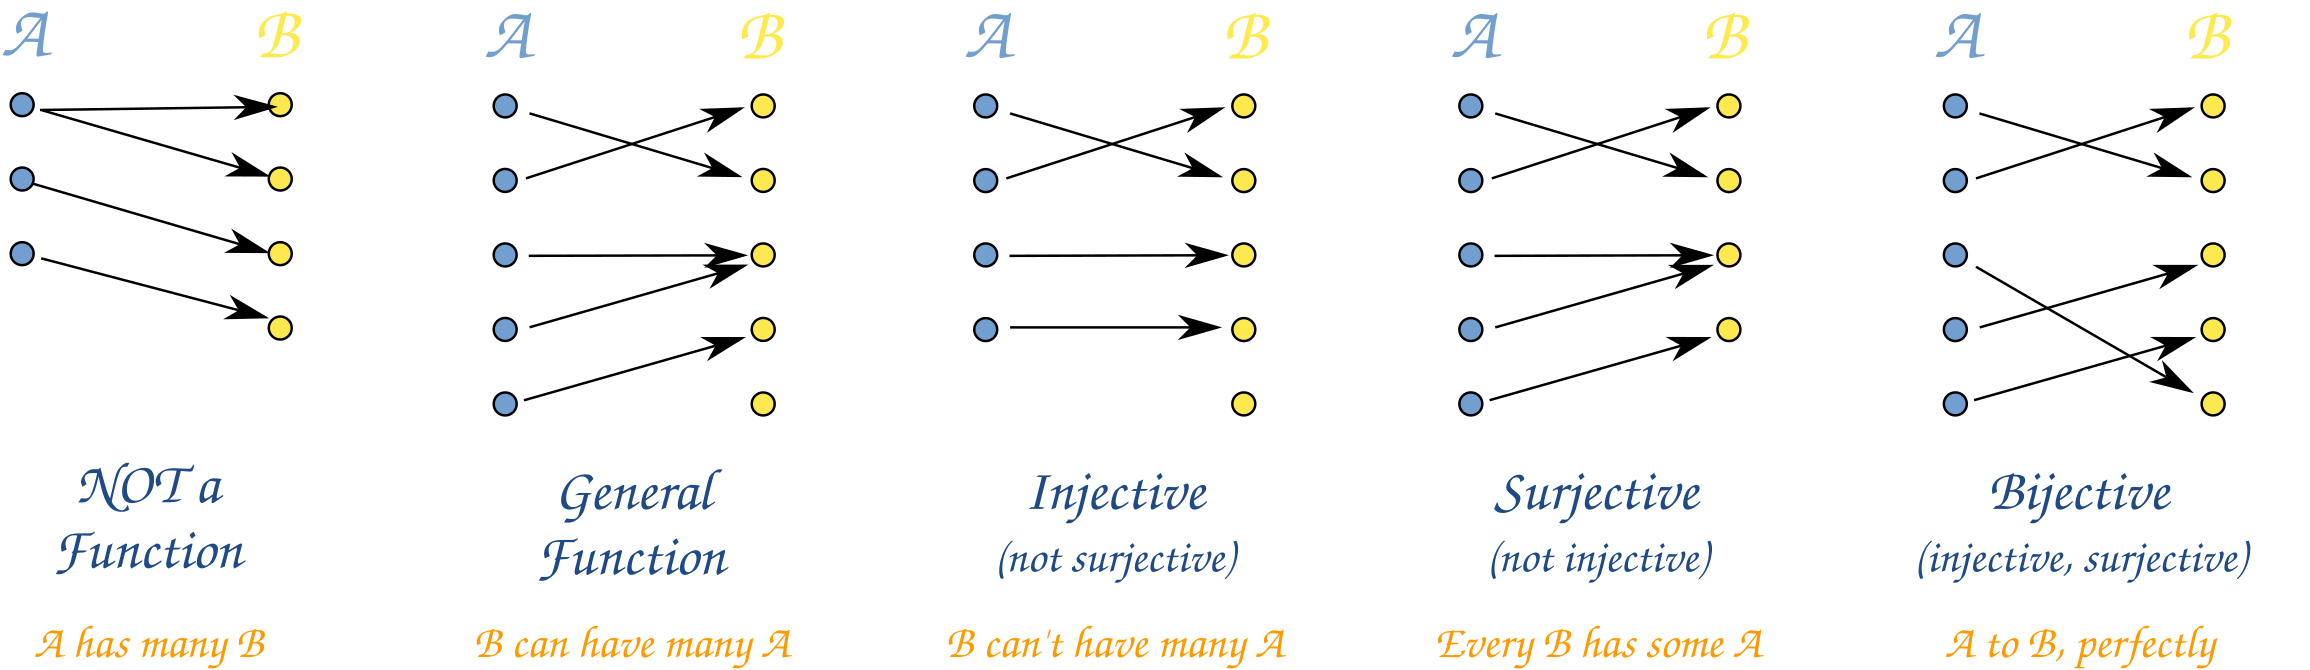
\includegraphics[scale=0.75]{function-mapping.png}
    \caption{Examples of the four types of functions, and a non-function. Source: Math is Fun.}
\end{figure}

One interesting observation you might make is that for $f:A\to B$ to be injective, $|A| \leq |B|$ must hold. Similarly, if $f:A\to B$ is surjective, $|A| \geq |B|$ must hold. Therefore if $f$ is bijective, $|A| = |B|$ must be true. For finite sets this isn't so remarkable, but later on in the course we will see how this gives us a method of comparing sets that are infinite in size! 

\section{Chinese Remainder Theorem}

I will first begin with the formal statement of the theorem. 
\begin{theorem}[Chinese Remainder Theorem] 
    Let $m_1, \dots, m_k$ be pairwise\footnote{Every pair of integers is relatively prime, as opposed to being relatively prime as a whole.} relatively prime positive integers, and let
    \[ M = m_1 \dots m_k.\]
    Then for every $k$-tuple $(x_1, \dots, x_k)$ of integers, there is exactly one residue class $x \pmod{M}$ such that
    \begin{align*}
        x &\equiv x_1 \pmod{m_1} \\ 
        x &\equiv x_2 \pmod{m_2} \\ 
          &\vdots  \\
        x &\equiv x_k \pmod{m_k}.
    \end{align*}
\end{theorem}

We call this a theorem, but it's really just a formalization of an intuition you should have. In other words, every integer mod $M$ can be uniquely identified by its values mod $m_1$, mod $m_2$, and so on. 

For example, knowing that $x\equiv 10 \pmod{15}$ is equivalent to knowing that $x\equiv 1\pmod{3}$ and $x \equiv 0 \pmod{5}$. The first condition restricts the possibilities to 5 different values (1, 4, 7, 10, 13), and the second condition tells you exactly which of these 5 the number is (10, being the only multiple of 5). You should expect this to happen in general.

\begin{example}
    Suppose we're trying to determine $8^{39} \pmod{15}$. Without using CRT, we're pretty much stuck with hand computation. But let's break this down mod 3 and mod 5. We have that 
    \[ 8^{39} \equiv (-1)^{39} \equiv -1 \equiv 2 \pmod{3} \] 
    and 
    \[ 8^{39} \equiv 3^{39} \equiv 3\cdot 9^{19} \equiv 3\cdot (-1)^{19} \equiv 2\pmod{5} \] 
    so by CRT, $8^{39}\equiv 2 \pmod{15}$. 
\end{example}

Extending the previous analogy, we can interpret this equivalence as understanding $x$ mod $M$ in terms of its basis vectors (1 mod $m_1$), (1 mod $m_2$), $\cdots$, (1 mod $m_k$). Each one specifies $x$'s value along that dimension (or that mod space). Then all we need to do is find out the correct coefficients to multiply each of the vectors by to create a linear combination that produces $x$ mod $M$. 

Let's create a general method for finding $x\mod{M}$ based on its values mod $m_1, \dots,$ mod $m_k$. Throughout this section, we will be using a fact that you have seen already, so we will refer to it by its common name. 

\begin{theorem}[Bezout's Lemma]
    Let $a,b$ be integers with $\gcd(a,b) = d$. Then there exists integers $x,y$ such that $ax+by = d$. Furthermore, all integers of the form $ax+by$ are multiples of $d$. 
\end{theorem}

First we will do a short, concrete example. 

\begin{example}[Dis 3B \#3]
    Let's find the $x$ for which 
    \begin{align*}
        x&\equiv 3 \pmod{11} \\ 
        x&\equiv 7 \pmod{13}.
    \end{align*}
    Recall that since $\gcd(11,13) = 1$, by Bezout's Lemma there are integers $a,b$ so that
    \[ x = 11a + 13b.\]
    We just need to pick them so that $x$ satisfies our above constraints (which will be unique mod 143 by CRT). First, let's take our equation mod 11 and use our constraint; this gives 
    \[ 3\equiv x \equiv 13b \pmod{11}.\] 
    So $b = 13^{-1}\times 3 \equiv 6\times 3 \equiv 7 \pmod{11}$. Now let's take our equation mod 13 and use the other constraint to get 
    \[ 7\equiv x \equiv 11a \pmod{13}.\] 
    So $a = 11^{-1}\times 7 \equiv 6\times 7 \equiv 3\pmod{13}$. Putting this all together, we find that 
    \[ x = 11a + 13b = 11\times 3 + 13\times 7 = 33 + 91 \implies  \boxed{x \equiv 124 \pmod{143}}.\] 
\end{example}

With this example in mind, let's see how we would carry out these steps in general. Suppose we have just two equations
    \begin{align*}
        x &\equiv x_1 \pmod{m_1} \\ 
        x &\equiv x_2 \pmod{m_2}.
    \end{align*}

    Since $\gcd(m_1, m_2) = 1$, by Bezout's Lemma there are integers $c_1, c_2$ for which 
    \[ x = c_1m_1 + c_2m_2\] 
    unique up to mod $m_1m_2$. Taking this mod $m_1$, we find 
    \[ x_1 \equiv x \equiv  c_2m_2 \pmod{m_1} \implies c_2 \equiv m_2^{-1} x_1 \pmod{m_1}.\]

    Taking the equation mod $m_2$, we also get 
    \[ x_2 \equiv x \equiv  c_1m_1 \pmod{m_2} \implies c_1 \equiv m_1^{-1} x_2 \pmod{m_2}.\]

    Putting this together, we find that 

    \[ \boxed{x \equiv (m_1)^{-1}_{m_2}m_1 x_2 + (m_2)^{-1}_{m_1}m_2 x_1 \pmod{m_1m_2}}\] 

    where $(a)^{-1}_m$ denotes $a^{-1}$ mod $m$. 

    This looks complicated, but remember that what we did was pretty natural. We simply had a system of equations with some constraints, and using those constraints we found out what each of the required coefficients are. 

    Having seen the case of two moduli, we can proceed with the general case. Let $M = m_1\dots m_k$ be a product of pairwise coprime integers, and suppose we have the system 
    \begin{align*}
        x &\equiv x_1 \pmod{m_1} \\ 
        x &\equiv x_2 \pmod{m_2} \\ 
          &\vdots  \\
        x &\equiv x_k \pmod{m_k}.
    \end{align*}
    
    Fix an $m_i$. Since $\gcd(M/m_i, m_i) = 1$, by Bezout's Lemma, there are integers $C_i, c_i$ for which 
    \[ x = C_i \left(\dfrac{M}{m_i}\right) + c_i m_i.\] 

    Taking this mod $m_i$, we find that 

    \[ x_i \equiv x \equiv C_i \left(\dfrac{M}{m_i}\right) \implies C_i \equiv \left(\dfrac{M}{m_i}\right)^{-1} x_i \pmod{m_i}.\] 

    I claim that these coefficients create a solution for $x$, i.e. that 
    \[ x = \sum_{i = 1}^k C_i \left(\dfrac{M}{m_i}\right) \equiv \sum_{i=1}^k \left(\dfrac{M}{m_i}\right)^{-1}_{m_i} \left(\dfrac{M}{m_i}\right) x_i \pmod{M}.\] 

    If I took this expression mod $m_i$, every term that's not the $x_i$ term would be 0 as $\frac{M}{m_j}$ would contain $m_i$. The $i$th term would cancel out to just $x_i$, which is precisely what we wanted. 

    In a sense, these coefficients are our ``basis coefficients'' which are always 1 mod $m_i$ and 0 otherwise, so that $x$ mod $m_i$ is always $x_i$. When we study Lagrange Interpolation, you will see a deep connection between these two concepts, as they are essentially the same idea applied in two different contexts. 


\subsection{Quick Remark}
Here's a quick and dirty way to solve Question 3. 
\begin{example}[Very, Very Fast]
    Let's find the $x$ for which 
    \begin{align*}
        x&\equiv 3 \pmod{11} \\ 
        x&\equiv 7 \pmod{13}.
    \end{align*}
    The second equation tells us that $x = 7 + 13k$ for some $k\in \ZZ$. If we take this equation mod 11, we know it must be equivalent to 3, so 
    \[ 3 \equiv x \equiv 7 + 2k \implies 2k \equiv 7\pmod{11}\] 
    from which it's easy to tell that $k = 9$. Thus, $x = 7 + 13\cdot 9 \equiv 128 \pmod{143}$ is our answer.
\end{example}

\end{document}
